\documentclass{standalone}
\usepackage{pgfplots}

\begin{document}

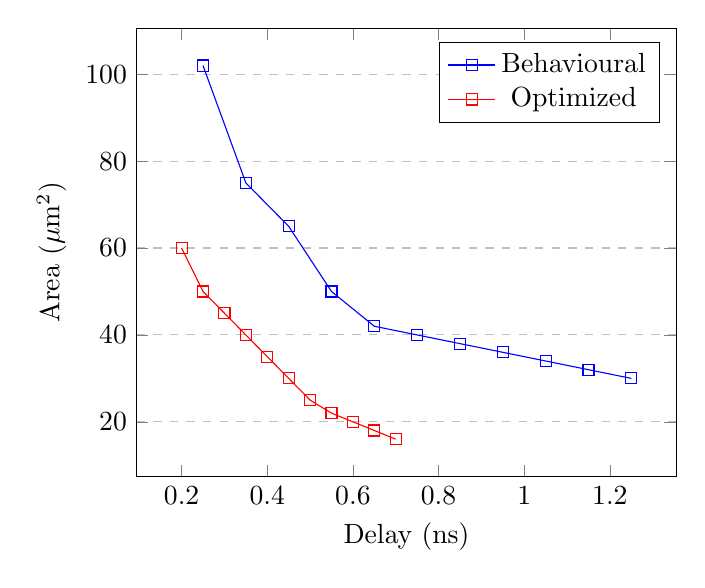
\begin{tikzpicture}
    \begin{axis}[
        xlabel={Delay (ns)},
        ylabel={Area ($\mu$m$^2$)},
        legend pos=north east,
        ymajorgrids=true,
        grid style=dashed,
    ]
    
    % Behavioral data points
    \addplot[
        color=blue,
        mark=square,
        ]
        coordinates {
            (0.25, 102)
            (0.35, 75)
            (0.45, 65)
            (0.55, 50)
            (0.65, 42)
            (0.75, 40)
            (0.85, 38)
            (0.95, 36)
            (1.05, 34)
            (1.15, 32)
            (1.25, 30)
        };
        \addlegendentry{Behavioural}
        
    % Optimized data points
    \addplot[
        color=red,
        mark=square,
        ]
        coordinates {
            (0.2, 60)
            (0.25, 50)
            (0.3, 45)
            (0.35, 40)
            (0.4, 35)
            (0.45, 30)
            (0.5, 25)
            (0.55, 22)
            (0.6, 20)
            (0.65, 18)
            (0.7, 16)
        };
        \addlegendentry{Optimized}
        
    \end{axis}
\end{tikzpicture}

\end{document}